\documentclass[
    a4paper,
    oneside,
    10pt
]{article}

\usepackage{lmodern}
\usepackage[utf8]{inputenc}
\usepackage[T1]{fontenc}
\usepackage[english]{babel}

\usepackage[
	bindingoffset = 0.2in,
	left = 0.5in,
	right = 0.5in,
	top = 0.5in,
	bottom = 0.5in,
	footskip = 0.25in
]{geometry}
\usepackage{courier}

\usepackage{calc}
\usepackage{fontawesome5}
\usepackage{makecell}
\usepackage{longtable}
\usepackage{tikz}
\usetikzlibrary{calc} 
\usepackage{xcolor}
\usepackage{hyperref}

\usepackage{graphicx}
\graphicspath{ {./db/} }

\newenvironment{timeline}{%
	\begin{longtable}{ c | c }%
}{%
	\end{longtable}%
}
\newcommand{\tldate}[1]{%
	\begin{minipage}[t]{2cm}%
		\begin{flushright}%
			\vspace{10pt}#1%
		\end{flushright}%
	\end{minipage}%
}
\newcommand{\tlcontent}[1]{%
	\begin{minipage}[t]{\textwidth-2cm}%
		\vspace{10pt}#1%
	\end{minipage}%
}
\newcommand{\lttitle}[1]{\textbf{\Large #1}\vspace{2pt}}
\newcommand{\ltsubtitle}[1]{\textbf{\large #1}\vspace{2pt}}
\newcommand{\ltloc}[1]{\textit{#1}}

\definecolor{progbarBgColor}{HTML}{101010}
\definecolor{progbarColor}{HTML}{606060}
\newcommand{\progress}[1]{%
	\begin{tikzpicture}%
		\fill[color=progbarColor] (0.0, 0.0) rectangle (#1*0.9*\linewidth, 0.15);
		\draw[color=progbarBgColor] (0.0, 0.0) rectangle (0.9*\linewidth, 0.15);
	\end{tikzpicture}%
}

\begin{document}

    %==================== HEADER ====================%
    \begin{tabular}{ @{} c m{12cm} @{} }
		\begin{tikzpicture}[baseline=(ola.center),inner sep=0pt]
			\clip (0,0)  circle (2cm) node (ola) {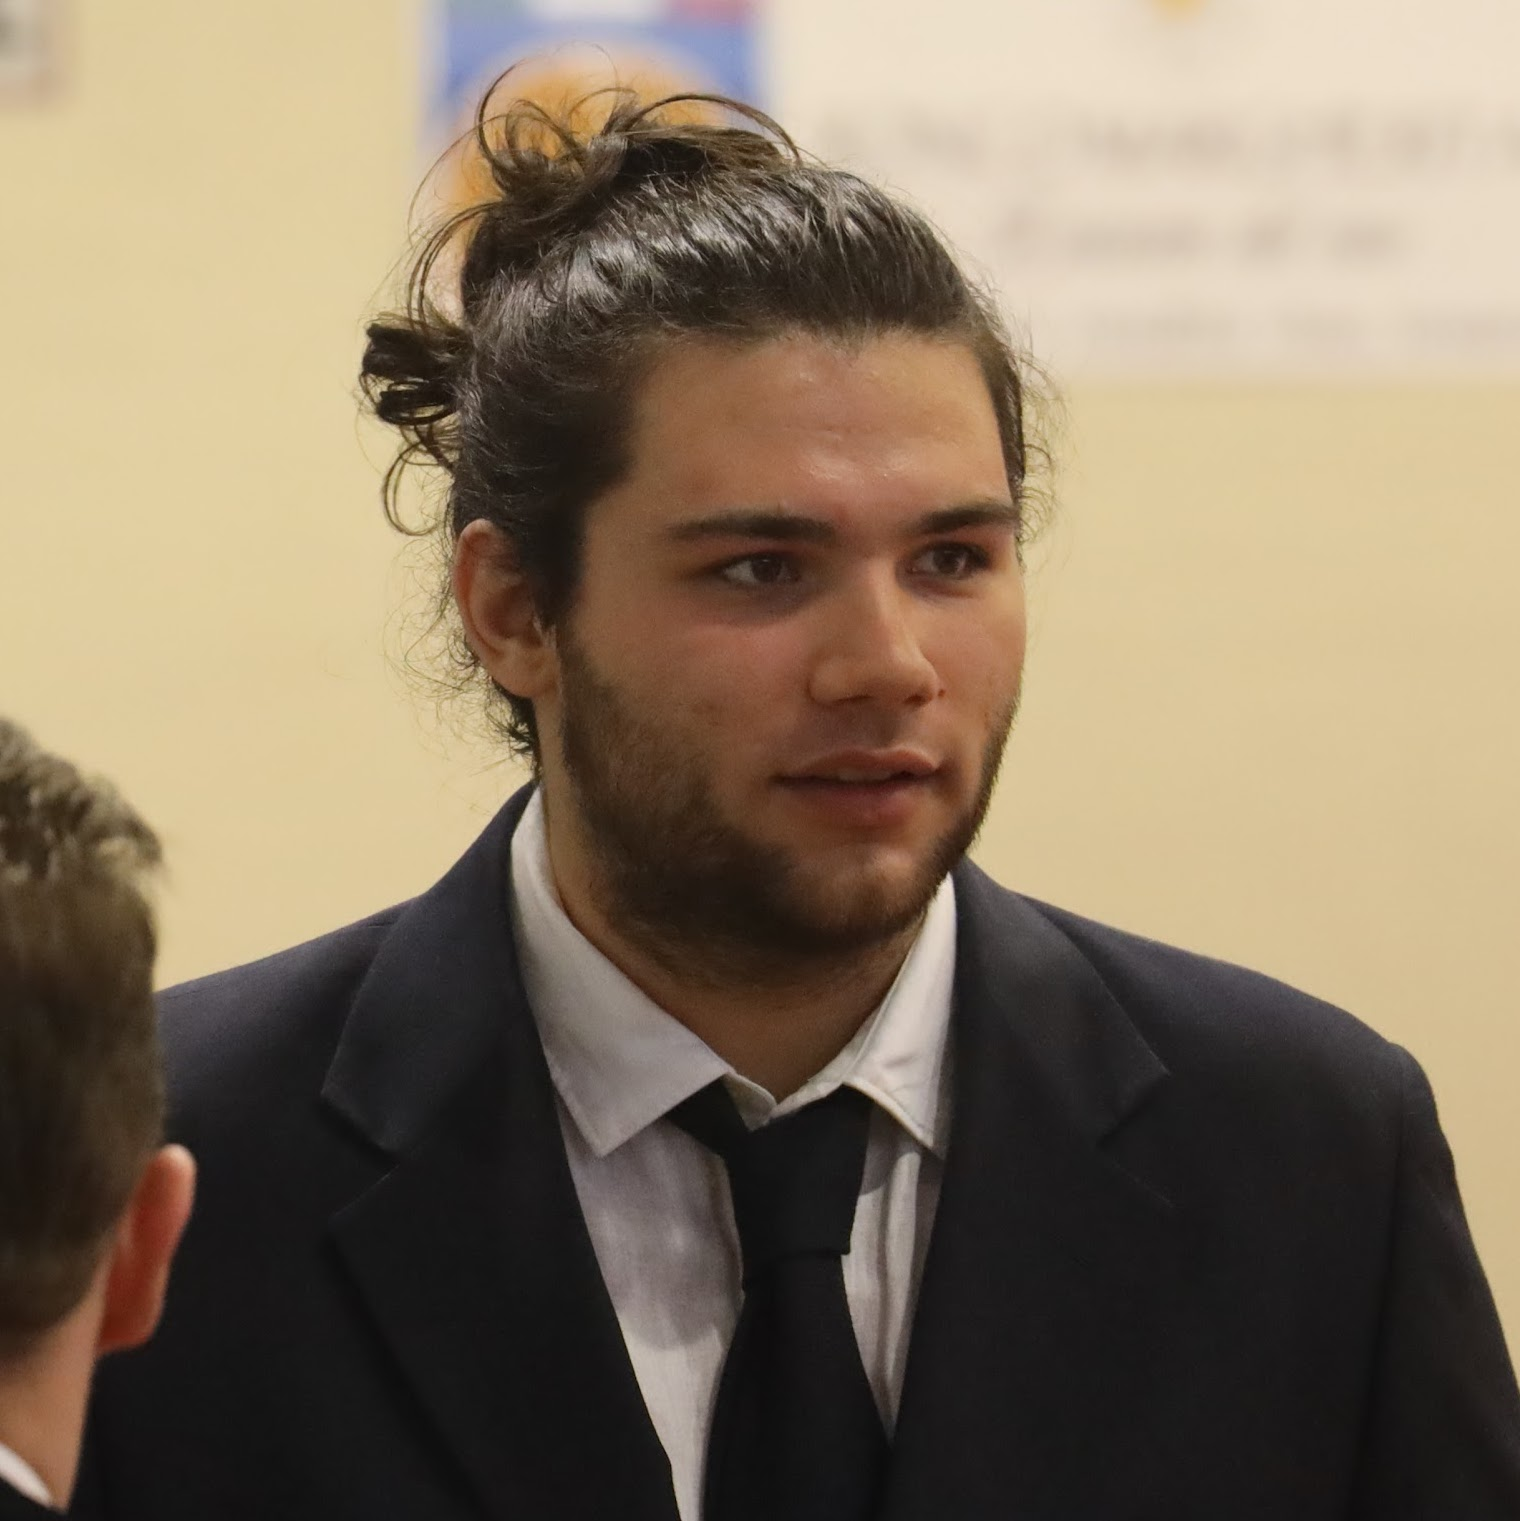
\includegraphics[height=4cm]{profile.jpg}};
		\end{tikzpicture} & \shortstack[l]{
			{\fontsize{25}{30}\selectfont\textbf{Urbani Ludovico}} \vspace{.3cm} \\
            {\fontsize{15}{20}\selectfont\textbf{Developer}}
		}
	\end{tabular} \\
	\begin{center}
		\begin{tabular}{ m{15cm} }
			\vspace{1cm} \\
			\hline
		\end{tabular}
	\end{center}
	\vspace{1cm}

    %==================== PROFILE ====================%

    \section{About}
	\begin{center}
		\renewcommand{\arraystretch}{1.25}
		\begin{tabular}{ r@{\hspace{.5cm}} | @{\hspace{.5cm}}l }
            Born & 2 June 2003 \\
			Fiscal Code & RBNLVC03H02L424F \\
			Living & Trieste (IT)
		\end{tabular}
	\end{center}

    \subsection{Contacts}
	\begin{center}
		\renewcommand{\arraystretch}{1.25}
		\begin{tabular}{ r@{\hspace{.5cm}} @{\hspace{.5cm}}l }
            \faAt & lu.urbani@outlook.com \\
			\faPhone & (+39) 331-2603770 \quad\faWhatsapp\;\faTelegram
		\end{tabular}
	\end{center}
	
    %==================== CONTENT ====================%
    
    \section{Skills}
    
    \subsection{Language Skills}
    \begin{itemize}
    		\item Italian \\ \progress{0.95}
    		\item English \\ \progress{0.7}
    		\item Latin \\ \progress{0.2}
    \end{itemize}
    
    \subsection{Digital Skills}
    
    \subsubsection{Development}
    \begin{itemize}
    		\input{|python3 api/skills_development.py}
    \end{itemize}
    
    \subsubsection{Operating Systems}
    \begin{itemize}
    		\input{|python3 api/skills_os.py}
    \end{itemize}
    
    \subsubsection{Programming Languages}
    \begin{itemize}
    		\input{|python3 api/skills_programming_languages.py}
    \end{itemize}
    
    \subsubsection{Software}
    \begin{itemize}
    		\input{|python3 api/skills_software.py}
    \end{itemize}
    
    \section{Education}
    \begin{timeline}
    		\input{|python3 api/education.py}
    \end{timeline}
    
    \subsection{Qualifications}
    \begin{timeline}
    		\input{|python3 api/qualifications.py}
    \end{timeline}
    
    \subsection{Conferences}
    \begin{timeline}
    		\input{|python3 api/conferences.py}
    \end{timeline}
    
    \section{Work Experience}
	\begin{timeline}
    		\input{|python3 api/work.py}
    \end{timeline}
    
    \subsection{Volunteering}
	\begin{timeline}
    		\input{|python3 api/volunteering.py}
    \end{timeline}
    
	\section{Honours and Awards}
    \begin{timeline}
    		\input{|python3 api/honours.py}
    \end{timeline}
    
    \section{Memberships}
    \begin{timeline}
    		\input{|python3 api/memberships.py}
    \end{timeline}
    
    \section{Administrative Roles}
    \begin{timeline}
    		\input{|python3 api/administrative_roles.py}
    \end{timeline}
    
    \section{Sport}
    	\subsection{Results}
    	\begin{timeline}
    		\input{|python3 api/sport_results.py}
    \end{timeline}
    
    \pagebreak
	\pagenumbering{roman}
    \tableofcontents

\end{document}